\section{块码}
\label{sec:dcc-block-codes}

一个比特直接送进翻转概率$p=0.1$的二元对称信道，出错的概率就是$0.1$。降低错误的朴素办法是重复：要发$0$就连发$000$，要发$1$就连发$111$，接收端看三个符号中哪个占多数。只有至少两个符号被翻转时才判错，这比单个符号翻转少见得多。

这个例子包含了信道编码的全部要素：消息不是逐个符号送出的，而是先被映成一整块输入；块中的冗余让接收端在部分符号出错时仍能判断发送的是哪条消息。本节把这些要素写成定义，规定码率与错误概率的口径。后面的容量定理和第~\ref{chap:channel-codes}章的具体纠错码都使用这里的口径。

\subsection{编码器与解码器}
\label{sec:dcc-encoder-decoder}

设要传送的消息取自有限集合$\{1,\dots,M\}$，信道使用$n$次。编码就是给每条消息指定一个长度为$n$的输入块，解码就是根据收到的输出块猜出消息。

\begin{definition}[块码]
\label{def:dcc-block-code}
离散信道上的一个$(M,n)$\term{块码}（block code）由两部分组成：
\begin{itemize}
 \item 编码器$f:\{1,\dots,M\}\to\mathcal{X}^n$，记$x^n(m)=f(m)$，称为消息$m$的码字，全部码字组成码本；
 \item 解码器$g:\mathcal{Y}^n\to\{1,\dots,M\}$，把每个输出块判为一条消息。
\end{itemize}
码的码率定义为
\begin{equation}
 R=\frac{\log_2M}{n}\quad\text{比特每次信道使用}.
 \label{eq:dcc-rate}
\end{equation}
\end{definition}

$\log_2M$是从$M$条消息中选出一条所需的比特数，除以$n$就是平均每次使用信道承载的比特数。码率最高为$\log_2\lvert\mathcal{X}\rvert$，此时$M=\lvert\mathcal{X}\rvert^n$，每个输入块都是码字，没有任何冗余。

\paragraph{三次重复码}
\term{重复码}（repetition code）中$M=2$，$n=3$。把消息记作$0$与$1$，码字是$000$与$111$，码率为$\tfrac13$。解码器采用\term{多数判决}（majority decoding）：输出块中$1$多于$0$时判为$1$，否则判为$0$。下面走一遍传输过程，区分四个对象：
\begin{enumerate}
 \item 消息：$m=1$，这是要传的内容；
 \item 码字：$x^3(1)=111$，这是送进信道的输入块；
 \item 输出块：信道翻转了第二位，接收端收到$y^3=101$；
 \item 判决：$101$中有两个$1$，$g(101)=1$，判决$\hat{m}=1$与消息一致。
\end{enumerate}
消息与判决属于消息集合，码字与输出块属于符号块；错误指的是判决与消息不同，而不是输出块与码字不同。这次传输中输出块有一位错了，判决仍然正确。

图~\ref{fig:dcc-repetition-cube}把长度为$3$的全部$8$个输出块画成立方体的顶点，相邻顶点只差一位。两个码字在相对的两个角上，多数判决把立方体分成两半：离$000$较近的四个顶点判为$0$，离$111$较近的四个判为$1$。从$111$出发翻转一位只能走到黄色顶点，所以单个翻转总能被纠正。

\begin{BookInlineFigure}
 \centering
 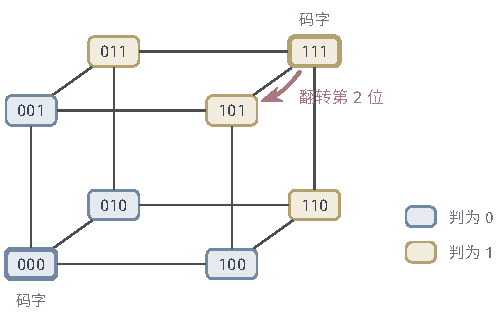
\includegraphics[width=85.4mm]{figures/07-probability/06-channel-coding/tikz/dcc-repetition-cube/figure.pdf}
 \caption{长度为$3$的输出块构成立方体的顶点，相邻顶点只差一位。粗框为码字$000$与$111$；蓝色顶点（至多一个$1$）判为$0$，黄色顶点（至少两个$1$）判为$1$。红色箭头是正文的例子：发送$111$，第二位翻转，收到$101$，判为$1$。}
 \label{fig:dcc-repetition-cube}
\end{BookInlineFigure}

在翻转概率$p=0.1$的二元对称信道上，发送$111$而判错，需要至少两位翻转。恰好两位翻转有$3$种位置，三位全翻有$1$种，所以
\[
 \mathbb{P}(\text{判错})=3p^2(1-p)+p^3=3\times0.01\times0.9+0.001=0.028 .
\]
由对称性，发送$000$时判错的概率也是$0.028$。

\paragraph{最好的解码器}
码本给定以后，解码器还可以自由选择。若每条消息以相同的概率$1/M$出现，判对的概率是
\[
 \frac1M\sum_{m=1}^{M}\ \sum_{y^n:\,g(y^n)=m}W^n\bigl(y^n\mid x^n(m)\bigr)
 =\frac1M\sum_{y^n\in\mathcal{Y}^n}W^n\bigl(y^n\mid x^n(g(y^n))\bigr) .
\]
右边对每个输出块分别求和，因此逐项取最大即可：对每个$y^n$，让$g(y^n)$取使$W^n(y^n\mid x^n(m))$最大的$m$（并列时任取其一）。这样的判决规则称为\term{最大似然解码}（maximum-likelihood decoding），它使均匀消息下的错误概率最小。在$p<\tfrac12$的二元对称信道上，$W^n(y^n\mid x^n)=p^{k}(1-p)^{n-k}$，其中$k$是$y^n$与$x^n$不同的位置数；因为$p/(1-p)<1$，似然随$k$增大而减小，最大似然就是选与输出块差异位置最少的码字。对重复码，这正是多数判决。

\subsection{错误概率与可达速率}
\label{sec:dcc-error-and-rates}

重复码的例子已经给出一个错误概率，但一般的码中，不同消息被判错的概率可以不同。为此先对每条消息定义条件错误概率，再用两种方式汇总。

\begin{definition}[错误概率]
\label{def:dcc-error-probabilities}
对$(M,n)$码，消息$m$的条件错误概率是
\begin{equation}
 \lambda_m=\mathbb{P}\bigl(g(Y^n)\neq m\mid X^n=x^n(m)\bigr)=\sum_{y^n:\,g(y^n)\neq m}W^n\bigl(y^n\mid x^n(m)\bigr) .
 \label{eq:dcc-lambda}
\end{equation}
\term{平均错误概率}（average error probability）与\term{最大错误概率}（maximal error probability）分别为
\begin{equation}
 P_{\mathrm{e}}=\frac1M\sum_{m=1}^{M}\lambda_m,\qquad \lambda_{\max}=\max_{1\leq m\leq M}\lambda_m .
 \label{eq:dcc-pe}
\end{equation}
\end{definition}

若消息$M$在$\{1,\dots,M\}$上均匀分布，$P_{\mathrm{e}}$就是判错的概率$\mathbb{P}(g(Y^n)\neq M)$。这里用同一字母$M$表示消息变量和消息个数，下文由上下文区分。$\lambda_{\max}$不依赖消息的分布，它保证每条消息都很少出错。平均不超过最大值，所以$P_{\mathrm{e}}\leq\lambda_{\max}$；第~\ref{sec:dcc-max-error}小节会说明，在渐近意义下两种口径给出相同的速率极限。

\paragraph{可达速率}
在二元对称信道这类每个输出块都可能来自任一码字的信道上，有限码的错误概率总是正的，所以“可靠”只能在码长增长的极限中定义：要求一列码的错误趋于零，同时码率不低于给定的值。

\begin{definition}[可达速率与容量]
\label{def:dcc-achievable}
称$R\geq0$为\term{可达速率}（achievable rate），若存在一列$(M_n,n)$码，满足
\begin{equation}
 M_n\geq2^{nR},\qquad \lim_{n\to\infty}P_{\mathrm{e}}^{(n)}=0 ,
 \label{eq:dcc-achievable}
\end{equation}
其中$P_{\mathrm{e}}^{(n)}$是第$n$个码的平均错误概率。可达速率的上确界称为信道的\term{信道容量}（channel capacity），记作$C_{\mathrm{op}}$。
\end{definition}

$R=0$总是可达的：取$M_n=1$，只有一条消息，解码器永远判对。可达速率的集合是区间：若$R$可达，比它小的速率用同一列码即可满足$M_n\geq2^{nR'}$。下标“op”表示这个容量是按传输任务定义的；下一节给出一个由信道直接计算的量，第~\ref{sec:dcc-coding-theorem}节证明二者相等。

\paragraph{重复码不够}
长度为奇数$n$的重复码在$p=0.1$的二元对称信道上，判错的概率是$\mathrm{Bin}(n,0.1)$至少取到$(n+1)/2$的概率。由第~\ref{chap:laws-of-large-numbers}章的弱大数律，翻转比例趋于$0.1<\tfrac12$，这个概率趋于零。可是码率$1/n$也趋于零，所以重复码只说明速率$0$可达。图~\ref{fig:dcc-repetition-error}画出前几个重复码：错误按指数下降，但它们在码率—错误平面上全部挤向纵轴，远离$C\approx0.531$。

\begin{BookInlineFigure}
 \centering
 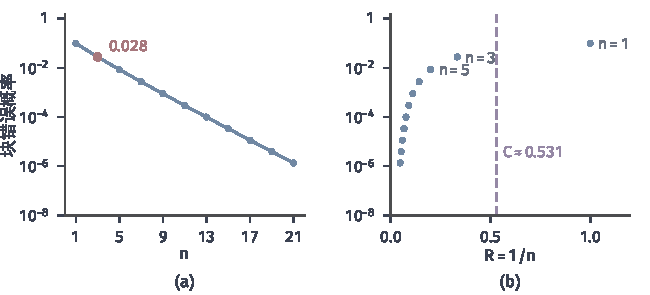
\includegraphics[width=110mm]{figures/07-probability/06-channel-coding/matplotlib/dcc-repetition-error/figure.pdf}
 \caption{翻转概率$0.1$的二元对称信道上，奇数长度$n$的重复码配合多数判决。(a) 块错误概率随$n$的精确值，对数坐标，红点为$n=3$时的$0.028$；(b) 同一组码在码率—错误平面上的位置，码率为$1/n$，紫色虚线为第~\ref{sec:dcc-bsc}小节算出的容量$0.531$。}
 \label{fig:dcc-repetition-error}
\end{BookInlineFigure}

图中$n=1$的“码”码率为$1$，超过了容量，错误概率却只有$0.1$。这并不矛盾：容量限制的是错误能否趋于零，对单个有限码的错误概率没有直接要求。反过来也一样，速率低于容量只保证存在错误趋于零的码列，并不保证某个有限长度的码错误为零。可达速率是关于码长增长时的极限陈述，有限长度需要多少冗余由第~\ref{chap:channel-codes}章讨论。
